\section{Results and analysis}\label{sec:results}

\subsection{Main results}\label{sec:main}

\begin{table}[!ht]
\caption{EX (\%) on BIRD dev and Spider test, overall and at each
difficulty level of the benchmark. Federated models are after
\setting{rounds.total} rounds, and centralized SFT after
\setting{central.epochs} epochs. Models marked ``second seed'' repeat
the training with another seed. $\Delta$ and $p$ compare each model with
FedAvg SFT of the same block. The $p$ is that of the exact McNemar test after the Holm correction, and
an asterisk marks a significant difference
(Section~\ref{sec:stat-test}). Bold marks the
highest value of each column within a block.}\label{tab:main}
\footnotesize
%% Written by tools/paper_numbers.py. Do not edit.
\setlength{\tabcolsep}{3.5pt}%
\begin{tabular}{@{}lrrrrrrl@{}}
\toprule
BIRD dev & EX & Simple & Moderate & Challenging &  & $\Delta$ & $p$ \\
\midrule
No training & 29.47 & 35.89 & 20.47 & 17.24 &  & $-$13.10 & $8.4\times10^{-27}$\textsuperscript{*} \\
Local SFT & -- & -- & -- & -- &  & -- & -- \\
Centralized SFT & -- & -- & -- & -- &  & -- & -- \\
FedAvg SFT & 42.57 & 51.35 & 29.96 & 26.90 &  &  &  \\
FedDPO & 45.50 & 52.54 & 35.99 & 31.03 &  & +2.93 & 0.014\textsuperscript{*} \\
\method & \textbf{48.76} & \textbf{56.00} & \textbf{39.66} & \textbf{31.72} &  & +6.19 & $2.3\times10^{-10}$\textsuperscript{*} \\
\method{} against centralized SFT &  &  &  &  &  & -- & -- \\
\midrule
Spider test & EX & Easy & Medium & Hard & Extra & $\Delta$ & $p$ \\
\midrule
No training & 68.05 & 87.45 & 71.41 & 59.18 & 45.94 & $-$6.66 & $8.6\times10^{-15}$\textsuperscript{*} \\
Centralized SFT & 75.03 & 91.06 & 78.30 & 67.17 & 56.30 & +0.32 & 0.69 \\
FedAvg SFT & 74.71 & 90.64 & 78.18 & 66.74 & 55.74 &  &  \\
FedDPO & -- & -- & -- & -- & -- & -- & -- \\
\method & \textbf{78.20} & \textbf{91.91} & \textbf{81.91} & \textbf{71.06} & \textbf{60.50} & +3.49 & $2.6\times10^{-6}$\textsuperscript{*} \\
\method{} against centralized SFT &  &  &  &  &  & +3.17 & $7.1\times10^{-5}$\textsuperscript{*} \\
\bottomrule
\end{tabular}

\end{table}

At \setting{rounds.total} rounds, \method{} is significantly above
FedAvg SFT on both benchmarks, by \gap{bird}{fedavg}{4}{k2}{4} EX points
on BIRD dev and \gap{spider}{fedavg}{4}{k2}{4} on Spider test, and it is
higher at every difficulty level, most of all on the moderate questions
of BIRD dev and on the extra-hard questions of Spider test
(Table~\ref{tab:main}). It is also significantly above FedDPO on BIRD
dev and centralized SFT on Spider test, and further rounds of FedAvg SFT
do not close the gap (Fig.~\ref{fig:rounds}).

\begin{figure}[!t]
\centering
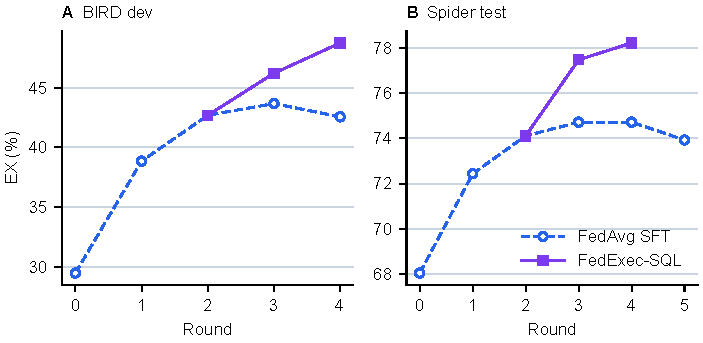
\includegraphics{figures/fig_rounds_cmc.pdf}
\caption{EX by round on \panel{a} BIRD dev and \panel{b} Spider test.
Round~0 is the pretrained model. \method{} continues from the FedAvg SFT
model of round~\setting{rounds.warmup}, and FedAvg SFT has a fifth round
on Spider test.}
\label{fig:rounds}
\end{figure}

FedAvg SFT does not improve after its third round on either benchmark.
On BIRD dev, its fourth round changes EX by
\gain{bird}{fedavg}{3}{fedavg}{4} points
($p = {}$\padj{bird}{fedavg}{3}{fedavg}{4}), and its highest EX,
\ex{bird}{fedavg}{3}\% after the third round, is
\gap{bird}{fedavg}{3}{k2}{4} points below \method{}
($p = {}$\padj{bird}{fedavg}{3}{k2}{4}). On Spider test, it stays at
\ex{spider}{fedavg}{3}\% after its third and fourth rounds and reaches
\ex{spider}{fedavg}{5}\% after a fifth
($p = {}$\padj{spider}{fedavg}{4}{fedavg}{5} against the fourth). With
this fifth round, FedAvg SFT uses more GPU time than \method{} does in
four (Section~\ref{sec:cost}), and \method{} is
\gap{spider}{fedavg}{5}{k2}{4} points above it
($p = {}$\padj{spider}{fedavg}{5}{k2}{4}).

From the same model after \setting{rounds.warmup} rounds, one preference
round adds more than one further round of FedAvg SFT, significantly so on
Spider test (Fig.~\ref{fig:rounds}). On BIRD dev, the preference round
adds \gap{bird}{fedavg}{2}{k2}{3} points
($p = {}$\padj{bird}{fedavg}{2}{k2}{3}) and the FedAvg SFT round
\gap{bird}{fedavg}{2}{fedavg}{3} ($p = {}$\padj{bird}{fedavg}{2}{fedavg}{3}),
and the two models after three rounds differ by
\gap{bird}{fedavg}{3}{k2}{3} points ($p = {}$\padj{bird}{fedavg}{3}{k2}{3}).
On Spider test, the two steps are \gap{spider}{fedavg}{2}{k2}{3}
($p = {}$\padj{spider}{fedavg}{2}{k2}{3}) and
\gap{spider}{fedavg}{2}{fedavg}{3} points
($p = {}$\padj{spider}{fedavg}{2}{fedavg}{3}), and the two models after
three rounds differ by \gap{spider}{fedavg}{3}{k2}{3} points
($p = {}$\padj{spider}{fedavg}{3}{k2}{3}). The preference round takes
more GPU time than the FedAvg SFT round in both setups
(Section~\ref{sec:cost}).

On Spider test, centralized SFT after \setting{central.epochs} epochs
does not differ significantly from FedAvg SFT, and \method{} is \gap{spider}{central}{3}{k2}{4} points above
it ($p = {}$\padj{spider}{central}{3}{k2}{4}).

FedDPO, trained on the fixed execution-labeled pairs of the first
preference round of \method, is \gap{bird}{feddpo}{4}{k2}{4} EX points
($p = {}$\padj{bird}{feddpo}{4}{k2}{4}) and \tsgap{bird}{feddpo}{4}{k2}{4}
TS points ($p = {}$\tspadj{bird}{feddpo}{4}{k2}{4}) below \method{} on
BIRD dev at \setting{rounds.total} rounds, where its TS is
\ts{bird}{feddpo}{4}\%. After the first of the two preference
rounds, FedDPO is below \method{} by a difference that is not
significant, and its second round adds \gain{bird}{feddpo}{3}{feddpo}{4}
points ($p = {}$\padj{bird}{feddpo}{3}{feddpo}{4}), less than the second
preference round of \method{} adds (Section~\ref{sec:ablation}). Against
FedAvg SFT, FedDPO is significantly higher under EX and does not differ
significantly under TS (\tsgain{bird}{fedavg}{4}{feddpo}{4} points,
$p = {}$\tspadj{bird}{fedavg}{4}{feddpo}{4}). Trained on these pairs,
FedDPO differs from \method{} in two components, the renewal of the pairs
and the reference model and the NLL term, and
Section~\ref{sec:ablation} gives the effect of each.

\subsection{Analysis of the predictions}\label{sec:analysis}

The gain over FedAvg SFT comes with about half as many execution errors,
while incorrect results do not fall (Fig.~\ref{fig:errors}). An
execution error is an incorrect prediction that fails to execute,
reaches the time limit or is cut at the token limit, and an incorrect
result is one that executes and returns another result than the gold
SQL query. At \setting{rounds.total} rounds, execution errors go from
\nerr{bird}{fedavg}{4} with FedAvg SFT to \nerr{bird}{k2}{4} with
\method{} on BIRD dev ($p = {}$\errpadj{bird}{fedavg}{4}{k2}{4}) and from
\nerr{spider}{fedavg}{4} to \nerr{spider}{k2}{4} on Spider test
($p = {}$\errpadj{spider}{fedavg}{4}{k2}{4}). Incorrect results are
slightly more numerous with \method{}, \nwr{bird}{k2}{4} against
\nwr{bird}{fedavg}{4} on BIRD dev and \nwr{spider}{k2}{4} against
\nwr{spider}{fedavg}{4} on Spider test, and neither difference is
significant ($p = {}$\wrpadj{bird}{fedavg}{4}{k2}{4} and
\wrpadj{spider}{fedavg}{4}{k2}{4}).

On BIRD dev, \method{} answers \nfix{bird}{fedavg}{4}{k2}{4} questions
correctly that FedAvg SFT does not, \fact{moved.bird.error.correct} of
them execution errors of FedAvg SFT and \fact{moved.bird.wrong.correct}
incorrect results, and FedAvg SFT answers \nbrk{bird}{fedavg}{4}{k2}{4}
that \method{} does not. Of the other execution errors of FedAvg SFT,
\fact{moved.bird.error.wrong} return an incorrect result with \method{}
and \fact{moved.bird.error.error} remain execution errors. On Spider
test, \method{} answers \nfix{spider}{fedavg}{4}{k2}{4} questions
correctly that FedAvg SFT does not, \fact{moved.spider.error.correct}
from execution errors and \fact{moved.spider.wrong.correct} from
incorrect results, and FedAvg SFT answers
\nbrk{spider}{fedavg}{4}{k2}{4} that \method{} does not. Of the other
execution errors of FedAvg SFT,
\fact{moved.spider.error.wrong} return an incorrect result and
\fact{moved.spider.error.error} remain.

The pairs that the clients train on contain both kinds of incorrect
query. The incorrect sample of a pair is a query that fails to execute
or exceeds the time limit in \fact{pairs.bird.pref1.neg_error_pct}\% of
the pairs of the first preference round on BIRD and in
\fact{pairs.spider.pref1.neg_error_pct}\% on Spider, and in
\fact{pairs.bird.pref2.neg_error_pct}\% and
\fact{pairs.spider.pref2.neg_error_pct}\% of those of the second. In the
other pairs, it executes and returns another result than the gold SQL
query.

Under both EX and TS, a large part of the gain on BIRD dev consists of
correct predictions that read other tables or columns than the gold SQL
query. We parse each query with sqlglot and collect the tables it reads
and the columns it reads, each with its table, over the main query and
all its subqueries, a column written without its table being assigned
through the schema. A prediction reads other tables or columns when
either set differs from that of the gold SQL query. A prediction that
sqlglot cannot parse counts among these, which concerns
\fact{form.bird.fedavg.4.unparsed} predictions of FedAvg SFT and
\fact{form.bird.k2.4.unparsed} of \method{} on BIRD dev at
\setting{rounds.total} rounds. Under EX, FedAvg SFT has
\fact{form.bird.fedavg.4.other_right} correct predictions of this kind on
BIRD dev after \setting{rounds.total} rounds, about as many as after its
second and third, and \method{} has \fact{form.bird.k2.3.other_right}
after its first preference round and \fact{form.bird.k2.4.other_right}
after its second, while correct predictions on the tables and columns of
the gold SQL query go from \fact{form.bird.fedavg.4.gold_right} to
\fact{form.bird.k2.4.gold_right}. Under the generated suite, the two
groups go from \fact{form.bird.fedavg.4.other_right_ts} to
\fact{form.bird.k2.4.other_right_ts} and from
\fact{form.bird.fedavg.4.gold_right_ts} to
\fact{form.bird.k2.4.gold_right_ts}. On Spider test at
\setting{rounds.total} rounds, FedAvg SFT has
\fact{form.spider.fedavg.4.other_right} correct predictions on other
tables or columns, as many as the pretrained model, and \method{} has
\fact{form.spider.k2.4.other_right}, and those on the tables and columns
of the gold SQL query go from \fact{form.spider.fedavg.4.gold_right} to
\fact{form.spider.k2.4.gold_right}.

EX establishes that a prediction returns the gold result on the
evaluation database only, and the generated suite of BIRD dev checks it
on the content variants. The suite rejects about a third of the
EX-correct predictions on other tables or columns for both models,
\fact{form.bird.fedavg.4.other_ts_fail_pct}\% for FedAvg SFT and
\fact{form.bird.k2.4.other_ts_fail_pct}\% for \method, against about a
tenth of those on the tables and columns of the gold SQL query,
\fact{form.bird.fedavg.4.gold_ts_fail_pct}\% and
\fact{form.bird.k2.4.gold_ts_fail_pct}\%. Among the former, the share
rejected is lower for \method{} than for FedAvg SFT, and among the
latter it is higher. As \method{} has more EX-correct predictions on
other tables or columns than FedAvg SFT, a part of its EX gain in this
group is not confirmed by the suite. The TS gain over FedAvg SFT, a
significant \tsgap{bird}{fedavg}{4}{k2}{4} points
(Table~\ref{tab:ablation}), is the figure that already excludes the
rejected predictions, \fact{ts.bird.fedavg.4.rejected} EX-correct
predictions of FedAvg SFT and \fact{ts.bird.k2.4.rejected} of \method{}
in all.

\subsection{Ablation study}\label{sec:ablation}

\begin{table}[!ht]
\caption{Ablation study. Each variant is compared with \method{} after
the same number of rounds: $\Delta$ and $p$ are against \method{} in
its block, with $p$ and the asterisk as in Table~\ref{tab:main}. TS on
BIRD dev uses the generated suite (Section~\ref{sec:datasets}). The
FedAvg SFT model after \setting{rounds.warmup} rounds, listed first, is
the start of every variant except those with another number of warm-up
rounds. ``Fixed pairs and reference'' keeps the preference pairs
and the reference model of the first preference round. ``Averaged by
questions'' and ``Averaged equally'' weight the server average by the
numbers of questions or equally instead of by the pair counts.
``Clients pooled'' runs the preference rounds on the union of the
clients' data.}\label{tab:ablation}
\footnotesize
%% Written by tools/paper_numbers.py. Do not edit.
\setlength{\tabcolsep}{3pt}%
\small
\begin{tabular}{@{}lrrlrrlrrl@{}}
\toprule
 & \multicolumn{6}{c}{BIRD dev} & \multicolumn{3}{c}{Spider test} \\
\cmidrule(lr){2-7}\cmidrule(lr){8-10}
 & EX & $\Delta$ & $p$ & TS & $\Delta$ & $p$ & EX & $\Delta$ & $p$ \\
\midrule
FedAvg SFT, 2 rounds & 42.70 &  &  & 36.11 &  &  & 74.10 &  &  \\
\midrule
\multicolumn{10}{@{}l}{\textit{4 rounds}} \\
\midrule
\method & 48.76 &  &  & 41.59 &  &  & 78.20 &  &  \\
FedAvg SFT & 42.57 & $-$6.19 & $1.8\times10^{-10}$\textsuperscript{*} & 36.70 & $-$4.89 & $7.9\times10^{-7}$\textsuperscript{*} & 74.71 & $-$3.49 & $1.9\times10^{-6}$\textsuperscript{*} \\
Fixed pairs and reference & 46.15 & $-$2.61 & 0.0091\textsuperscript{*} & 39.05 & $-$2.54 & 0.0093\textsuperscript{*} & 78.02 & $-$0.18 & 1.00 \\
No NLL term & -- & -- & -- & -- & -- & -- &  &  &  \\
No preference term & 45.24 & $-$3.52 & $9.3\times10^{-4}$\textsuperscript{*} & 38.20 & $-$3.39 & 0.0015\textsuperscript{*} & -- & -- & -- \\
No warm-up round & -- & -- & -- & -- & -- & -- & 78.02 & $-$0.18 & 1.00 \\
Three warm-up rounds & -- & -- & -- & -- & -- & -- & 77.97 & $-$0.23 & 1.00 \\
Clients pooled &  &  &  &  &  &  & -- & -- & -- \\
\midrule
\multicolumn{10}{@{}l}{\textit{3 rounds}} \\
\midrule
\method & 46.22 &  &  & 39.05 &  &  & 77.46 &  &  \\
No NLL term & 44.98 & $-$1.24 & 1.00 & 38.92 & $-$0.13 & 1.00 & 73.59 & $-$3.87 & $1.5\times10^{-7}$\textsuperscript{*} \\
No preference term & 44.39 & $-$1.83 & 0.74 & 37.35 & $-$1.70 & 0.75 & 75.87 & $-$1.59 & 0.21 \\
Averaged by questions & 46.22 & +0.00 & 1.00 & 39.31 & +0.26 & 1.00 & 77.78 & +0.32 & 1.00 \\
Averaged equally & 46.02 & $-$0.20 & 1.00 & 38.92 & $-$0.13 & 1.00 & 76.94 & $-$0.52 & 0.98 \\
\bottomrule
\end{tabular}

\end{table}

Table~\ref{tab:ablation} removes or changes one component of \method{}
at a time, in the order of Section~\ref{sec:method}, and compares every
variant with \method{} after the same number of rounds. On BIRD dev
after \setting{rounds.total} rounds, EX and TS are significantly lower
without the renewal of the pairs and the reference model and without the
preference term. Without the NLL term, EX after one preference round is
significantly lower on Spider test, and neither the number of warm-up
rounds on Spider test nor the weights of the server average change EX
significantly.

Of the \setting{rounds.total} rounds, \method{} has
\setting{rounds.warmup} warm-up rounds and \setting{rounds.pref}
preference rounds, the variant without warm-up has four preference
rounds, and the variant with three warm-up rounds has one. On Spider,
warm-up lowers the number of questions that yield pairs, as more
questions have correct samples only (Section~\ref{sec:warmup}), and
without it TS is lower on the three sets of Section~\ref{sec:perturbed}
that have a suite, significantly on Spider-Syn.

With \setting{rounds.pref} preference rounds, the renewal of the pairs
and the reference model takes place once, at the second preference
round. The variant with fixed pairs and reference trains this round on
the pairs and with the reference model of the first, whereas \method{}
trains it on pairs built from new samples, which come from fewer
questions (Table~\ref{tab:cost}), with the global model of that round as
reference. The comparison covers the new pairs and the new reference
model together and does not separate them. The variant is
\gap{bird}{k2}{4}{fixed}{4} EX points below \method{} on BIRD dev and
does not differ significantly from it on Spider test. The second
preference round itself adds \gap{bird}{k2}{3}{k2}{4} points on BIRD dev
($p = {}$\padj{bird}{k2}{3}{k2}{4}) and a smaller step of
\gap{spider}{k2}{3}{k2}{4} points on Spider test that is not
significant ($p = {}$\padj{spider}{k2}{3}{k2}{4}).

In the one setting we tested, pairs of the gold SQL query with an
incorrect sample, for the questions without a correct sample, do not
raise EX. The setting is BIRD without warm-up rounds, over one preference
round from the same samples and labels. For each of the
\fact{warmup.bird.k0.no_correct} questions without a correct sample, the
variant adds \setting{pref.pairs} pairs of the gold SQL query with
incorrect samples drawn as in Section~\ref{sec:pairs}. With them, EX on
BIRD dev is \gap{bird}{k0}{1}{k0gold}{1} points lower,
\ex{bird}{k0gold}{1}\% against \ex{bird}{k0}{1}\%, a difference that is
not significant ($p = {}$\padj{bird}{k0}{1}{k0gold}{1}), execution
errors fall from \nerr{bird}{k0}{1} to \nerr{bird}{k0gold}{1}, and
incorrect results rise from \nwr{bird}{k0}{1} to \nwr{bird}{k0gold}{1}.

Without the preference term, a preference round trains with the NLL term
alone, on the correct sample of each pair. The variant still uses the
execution labels, since it trains on samples that return the gold
result: it is a form of rejection sampling
fine-tuning~\cite{yuan2023rft} in federated rounds. On BIRD dev after
\setting{rounds.total} rounds, it is \gap{bird}{fedavg}{4}{rft}{4} EX
points above FedAvg SFT ($p = {}$\padj{bird}{fedavg}{4}{rft}{4}) and
\gap{bird}{k2}{4}{rft}{4} EX points below \method{}. It ends with
\nerr{bird}{rft}{4} execution errors against \nerr{bird}{k2}{4} for \method{}
($p = {}$\errpadj{bird}{k2}{4}{rft}{4}) and with \nwr{bird}{rft}{4}
incorrect results against \nwr{bird}{k2}{4}, a difference that is not
significant after the correction
($p = {}$\wrpadj{bird}{k2}{4}{rft}{4}). After one preference round, its
EX does not differ significantly from that of \method{} on either
benchmark, whereas its execution errors are significantly more numerous:
\nerr{bird}{rft}{3} against \nerr{bird}{k2}{3} on BIRD dev
($p = {}$\errpadj{bird}{k2}{3}{rft}{3}) and \nerr{spider}{rft}{3}
against \nerr{spider}{k2}{3} on Spider test
($p = {}$\errpadj{spider}{k2}{3}{rft}{3}).

The first preference round without the NLL term, which is also the
first round of FedDPO, is \gap{spider}{k2}{3}{feddpo}{3} EX points below
\method{} on Spider test after the same round, and at
\ex{spider}{feddpo}{3}\% it is below the \ex{spider}{fedavg}{2}\% of
the model it starts from, a difference that we did not test. On BIRD dev, neither its EX nor its TS differs significantly from that of
\method{}, and it is \gap{bird}{fedavg}{2}{feddpo}{3} EX points above
its starting model, also not significantly
($p = {}$\padj{bird}{fedavg}{2}{feddpo}{3}). With the pairs and the
reference model of the first preference round kept, the NLL term changes
EX on BIRD dev after \setting{rounds.total} rounds by
\gain{bird}{feddpo}{4}{fixed}{4} points
($p = {}$\padj{bird}{feddpo}{4}{fixed}{4}).

Averaging by the numbers of questions or equally instead of by the pair
counts moves EX after one preference round by at most
\gap{bird}{k2}{3}{reagge}{3} points on BIRD dev and
\gap{spider}{k2}{3}{reagge}{3} on Spider test.

\subsection{Other models and federated setups}\label{sec:breadth}

\begin{table}[!ht]
\caption{EX (\%) of three models after \setting{rounds.total} rounds in
the main setup of each benchmark: the pretrained model (No training),
FedAvg SFT and \method. $\Delta$ and $p$ compare \method{} with FedAvg
SFT, as in Table~\ref{tab:main}.}\label{tab:models}
\footnotesize
%% Written by tools/paper_numbers.py. Do not edit.
\setlength{\tabcolsep}{3.5pt}%
\begin{tabular}{@{}lrrrrl@{}}
\toprule
Model & No training & FedAvg SFT & \method & $\Delta$ & $p$ \\
\midrule
Qwen2.5-Coder-1.5B & 68.05 & 74.71 & 78.20 & +3.49 & $1.9\times10^{-6}$\textsuperscript{*} \\
Qwen2.5-Coder-0.5B & 54.40 & 64.09 & 66.19 & +2.10 & 0.0056\textsuperscript{*} \\
DeepSeek-Coder-1.3B & 55.85 & -- & -- & -- & -- \\
\bottomrule
\end{tabular}

\end{table}

\begin{table}[!ht]
\caption{EX (\%) of FedAvg SFT and \method{} after \setting{rounds.total}
rounds in the federated setups of Table~\ref{tab:setups}, each evaluated
on the evaluation set of its benchmark. $\Delta$ and $p$ as in
Table~\ref{tab:main}.}\label{tab:federated}
\footnotesize
%% Written by tools/paper_numbers.py. Do not edit.
\setlength{\tabcolsep}{3.5pt}%
\begin{tabular}{@{}llrlrrrl@{}}
\toprule
Clients' data & Partition & Clients & Evaluated on & FedAvg SFT & \method & $\Delta$ & $p$ \\
\midrule
BIRD train & $\alpha=0.1$ & 5 & BIRD dev & 42.57 & 48.76 & +6.19 & $2.3\times10^{-10}$\textsuperscript{*} \\
Spider train & $\alpha=0.1$ & 5 & Spider test & 74.71 & 78.20 & +3.49 & $2.6\times10^{-6}$\textsuperscript{*} \\
Spider train & $\alpha=0.5$ & 5 & Spider test & -- & -- & -- & -- \\
Spider train & IID & 5 & Spider test & -- & -- & -- & -- \\
Spider train & $\alpha=0.5$ & 10 & Spider test & -- & -- & -- & -- \\
\bottomrule
\end{tabular}

\end{table}

On Spider test, \method{} is also significantly above FedAvg SFT with a
smaller model, by a smaller margin (Table~\ref{tab:models}):
\gap[qwen05]{spider}{fedavg}{4}{k2}{4} EX points with
\fact{model.qwen05}-Instruct. Table~\ref{tab:federated} repeats the
comparison in the three other partitions of Spider train
(Section~\ref{sec:fed-setups}).

\subsection{Perturbed questions}\label{sec:perturbed}

On Spider dev and the three sets built from Spider, \method{} is above
FedAvg SFT under EX and, where a suite exists, under TS, by
\tsgap{spiderdev}{fedavg}{4}{k2}{4} to \gap{dk}{fedavg}{4}{k2}{4} points,
and the differences are significant on Spider-Syn only
(Table~\ref{tab:robust}). Both models lose EX from Spider dev to
Spider-Syn, FedAvg SFT from \ex{spiderdev}{fedavg}{4}\% to
\ex{syn}{fedavg}{4}\% and \method{} from \ex{spiderdev}{k2}{4}\% to
\ex{syn}{k2}{4}\%.

Without warm-up rounds, the EX gain of \method{} over FedAvg SFT does not
appear under TS: the variant is above FedAvg SFT under EX on all four
sets, and on the three sets with a suite its TS is not above that of
FedAvg SFT. With \setting{rounds.warmup} warm-up rounds, EX on these
three sets does not differ significantly from that of the variant, and
TS is higher by \tsgap{spiderdev}{k0}{4}{k2}{4} to
\tsgap{realistic}{k0}{4}{k2}{4} points, significantly on Spider-Syn only.
On Spider-DK, EX is higher without warm-up, by a difference that is not
significant.

\subsection{Computation and communication cost}\label{sec:cost}

\begin{table}[!ht]
\caption{Cost of a round in the two main setups, summed over the
\fact{split.bird.a0.1.k5.clients} clients run one after another on one
GPU. ``Trained on'' gives the questions of a FedAvg SFT round and, in a
preference round, the questions that yield pairs and their pairs. GPU
minutes cover sampling and training. Labeling minutes are the elapsed
time of executing the samples on \setting{pref.label_threads} processor
threads and are not part of the GPU minutes. ``Sent'' is what a client
uploads in the round.}\label{tab:cost}
\footnotesize
%% Written by tools/paper_numbers.py. Do not edit.
\setlength{\tabcolsep}{3.5pt}%
\begin{tabular}{@{}llrrrrr@{}}
\toprule
 &  & \multicolumn{4}{c}{Minutes per round} &  \\
\cmidrule(lr){3-6}
Clients' data & Round & Sampling & Labels & Training & Total & Sent (MB) \\
\midrule
BIRD train & FedAvg SFT &  &  & 173 & 173 & 73.9 \\
 & Preference round 1 & 28 & 159 & 283 & 470 & 73.9 \\
 & Preference round 2 & 28 & 168 & 195 & 391 & 73.9 \\
\midrule
Spider train & FedAvg SFT &  &  & 124 & 124 & 73.9 \\
 & Preference round 1 & 18 & 3 & 182 & 203 & 73.9 \\
 & Preference round 2 & 19 & 3 & 88 & 109 & 73.9 \\
\bottomrule
\end{tabular}

\end{table}

A preference round adds client computation and no communication
(Table~\ref{tab:cost}). In every round of either kind, a client uploads
one adapter of \setting{adapter.mb} and one integer. The two preference
rounds take \fact{cost.bird.pref1.gpu_ratio} and
\fact{cost.bird.pref2.gpu_ratio} times the GPU minutes of a FedAvg SFT
round on BIRD and \fact{cost.spider.pref1.gpu_ratio} and
\fact{cost.spider.pref2.gpu_ratio} times on Spider, and training in the
second is shorter than in the first, as fewer questions yield pairs.
Over \setting{rounds.total} rounds, \method{} takes
\fact{cost.bird.k2.gpu_total} GPU minutes on BIRD against
\fact{cost.bird.fedavg4.gpu_total} for FedAvg SFT, and
\fact{cost.spider.k2.gpu_total} against
\fact{cost.spider.fedavg4.gpu_total} on Spider, where five rounds of
FedAvg SFT take \fact{cost.spider.fedavg5.gpu_total}. Labeling the
samples on \setting{pref.label_threads} processor threads adds elapsed
time, which we report apart from the GPU time.
